
%% bare_conf.tex
%% V1.3
%% 2007/01/11
%% by Michael Shell
%% See:
%% http://www.michaelshell.org/
%% for current contact information.
%%
%% This is a skeleton file demonstrating the use of IEEEtran.cls
%% (requires IEEEtran.cls version 1.7 or later) with an IEEE conference paper.
%%
%% Support sites:
%% http://www.michaelshell.org/tex/ieeetran/
%% http://www.ctan.org/tex-archive/macros/latex/contrib/IEEEtran/
%% and
%% http://www.ieee.org/

%%*************************************************************************
%% Legal Notice:
%% This code is offered as-is without any warranty either expressed or
%% implied; without even the implied warranty of MERCHANTABILITY or
%% FITNESS FOR A PARTICULAR PURPOSE! 
%% User assumes all risk.
%% In no event shall IEEE or any contributor to this code be liable for
%% any damages or losses, including, but not limited to, incidental,
%% consequential, or any other damages, resulting from the use or misuse
%% of any information contained here.
%%
%% All comments are the opinions of their respective authors and are not
%% necessarily endorsed by the IEEE.
%%
%% This work is distributed under the LaTeX Project Public License (LPPL)
%% ( http://www.latex-project.org/ ) version 1.3, and may be freely used,
%% distributed and modified. A copy of the LPPL, version 1.3, is included
%% in the base LaTeX documentation of all distributions of LaTeX released
%% 2003/12/01 or later.
%% Retain all contribution notices and credits.
%% ** Modified files should be clearly indicated as such, including  **
%% ** renaming them and changing author support contact information. **
%%
%% File list of work: IEEEtran.cls, IEEEtran_HOWTO.pdf, bare_adv.tex,
%%                    bare_conf.tex, bare_jrnl.tex, bare_jrnl_compsoc.tex
%%*************************************************************************

% *** Authors should verify (and, if needed, correct) their LaTeX system  ***
% *** with the testflow diagnostic prior to trusting their LaTeX platform ***
% *** with production work. IEEE's font choices can trigger bugs that do  ***
% *** not appear when using other class files.                            ***
% The testflow support page is at:
% http://www.michaelshell.org/tex/testflow/



% Note that the a4paper option is mainly intended so that authors in
% countries using A4 can easily print to A4 and see how their papers will
% look in print - the typesetting of the document will not typically be
% affected with changes in paper size (but the bottom and side margins will).
% Use the testflow package mentioned above to verify correct handling of
% both paper sizes by the user's LaTeX system.
%
% Also note that the "draftcls" or "draftclsnofoot", not "draft", option
% should be used if it is desired that the figures are to be displayed in
% draft mode.
%
\documentclass[conference]{IEEEtran}
% Add the compsoc option for Computer Society conferences.
%
% If IEEEtran.cls has not been installed into the LaTeX system files,
% manually specify the path to it like:
% \documentclass[conference]{../sty/IEEEtran}





% Some very useful LaTeX packages include:
% (uncomment the ones you want to load)


% *** MISC UTILITY PACKAGES ***
%
%\usepackage{ifpdf}
% Heiko Oberdiek's ifpdf.sty is very useful if you need conditional
% compilation based on whether the output is pdf or dvi.
% usage:
% \ifpdf
%   % pdf code
% \else
%   % dvi code
% \fi
% The latest version of ifpdf.sty can be obtained from:
% http://www.ctan.org/tex-archive/macros/latex/contrib/oberdiek/
% Also, note that IEEEtran.cls V1.7 and later provides a builtin
% \ifCLASSINFOpdf conditional that works the same way.
% When switching from latex to pdflatex and vice-versa, the compiler may
% have to be run twice to clear warning/error messages.






% *** CITATION PACKAGES ***
%
\usepackage{cite}
% cite.sty was written by Donald Arseneau
% V1.6 and later of IEEEtran pre-defines the format of the cite.sty package
% \cite{} output to follow that of IEEE. Loading the cite package will
% result in citation numbers being automatically sorted and properly
% "compressed/ranged". e.g., [1], [9], [2], [7], [5], [6] without using
% cite.sty will become [1], [2], [5]--[7], [9] using cite.sty. cite.sty's
% \cite will automatically add leading space, if needed. Use cite.sty's
% noadjust option (cite.sty V3.8 and later) if you want to turn this off.
% cite.sty is already installed on most LaTeX systems. Be sure and use
% version 4.0 (2003-05-27) and later if using hyperref.sty. cite.sty does
% not currently provide for hyperlinked citations.
% The latest version can be obtained at:
% http://www.ctan.org/tex-archive/macros/latex/contrib/cite/
% The documentation is contained in the cite.sty file itself.






% *** GRAPHICS RELATED PACKAGES ***
%
\ifCLASSINFOpdf
  \usepackage[pdftex]{graphicx}
  % declare the path(s) where your graphic files are
  % \graphicspath{{../pdf/}{../jpeg/}}
  % and their extensions so you won't have to specify these with
  % every instance of \includegraphics
  % \DeclareGraphicsExtensions{.pdf,.jpeg,.png}
\else
  % or other class option (dvipsone, dvipdf, if not using dvips). graphicx
  % will default to the driver specified in the system graphics.cfg if no
  % driver is specified.
  \usepackage[dvips]{graphicx}
  % declare the path(s) where your graphic files are
  % \graphicspath{{../eps/}}
  % and their extensions so you won't have to specify these with
  % every instance of \includegraphics
  % \DeclareGraphicsExtensions{.eps}
\fi
% graphicx was written by David Carlisle and Sebastian Rahtz. It is
% required if you want graphics, photos, etc. graphicx.sty is already
% installed on most LaTeX systems. The latest version and documentation can
% be obtained at: 
% http://www.ctan.org/tex-archive/macros/latex/required/graphics/
% Another good source of documentation is "Using Imported Graphics in
% LaTeX2e" by Keith Reckdahl which can be found as epslatex.ps or
% epslatex.pdf at: http://www.ctan.org/tex-archive/info/
%
% latex, and pdflatex in dvi mode, support graphics in encapsulated
% postscript (.eps) format. pdflatex in pdf mode supports graphics
% in .pdf, .jpeg, .png and .mps (metapost) formats. Users should ensure
% that all non-photo figures use a vector format (.eps, .pdf, .mps) and
% not a bitmapped formats (.jpeg, .png). IEEE frowns on bitmapped formats
% which can result in "jaggedy"/blurry rendering of lines and letters as
% well as large increases in file sizes.
%
% You can find documentation about the pdfTeX application at:
% http://www.tug.org/applications/pdftex





% *** MATH PACKAGES ***
%
%\usepackage[cmex10]{amsmath}
% A popular package from the American Mathematical Society that provides
% many useful and powerful commands for dealing with mathematics. If using
% it, be sure to load this package with the cmex10 option to ensure that
% only type 1 fonts will utilized at all point sizes. Without this option,
% it is possible that some math symbols, particularly those within
% footnotes, will be rendered in bitmap form which will result in a
% document that can not be IEEE Xplore compliant!
%
% Also, note that the amsmath package sets \interdisplaylinepenalty to 10000
% thus preventing page breaks from occurring within multiline equations. Use:
%\interdisplaylinepenalty=2500
% after loading amsmath to restore such page breaks as IEEEtran.cls normally
% does. amsmath.sty is already installed on most LaTeX systems. The latest
% version and documentation can be obtained at:
% http://www.ctan.org/tex-archive/macros/latex/required/amslatex/math/





% *** SPECIALIZED LIST PACKAGES ***
%
%\usepackage{algorithmic}
% algorithmic.sty was written by Peter Williams and Rogerio Brito.
% This package provides an algorithmic environment fo describing algorithms.
% You can use the algorithmic environment in-text or within a figure
% environment to provide for a floating algorithm. Do NOT use the algorithm
% floating environment provided by algorithm.sty (by the same authors) or
% algorithm2e.sty (by Christophe Fiorio) as IEEE does not use dedicated
% algorithm float types and packages that provide these will not provide
% correct IEEE style captions. The latest version and documentation of
% algorithmic.sty can be obtained at:
% http://www.ctan.org/tex-archive/macros/latex/contrib/algorithms/
% There is also a support site at:
% http://algorithms.berlios.de/index.html
% Also of interest may be the (relatively newer and more customizable)
% algorithmicx.sty package by Szasz Janos:
% http://www.ctan.org/tex-archive/macros/latex/contrib/algorithmicx/




% *** ALIGNMENT PACKAGES ***
%
\usepackage{array}
% Frank Mittelbach's and David Carlisle's array.sty patches and improves
% the standard LaTeX2e array and tabular environments to provide better
% appearance and additional user controls. As the default LaTeX2e table
% generation code is lacking to the point of almost being broken with
% respect to the quality of the end results, all users are strongly
% advised to use an enhanced (at the very least that provided by array.sty)
% set of table tools. array.sty is already installed on most systems. The
% latest version and documentation can be obtained at:
% http://www.ctan.org/tex-archive/macros/latex/required/tools/


%\usepackage{mdwmath}
%\usepackage{mdwtab}
% Also highly recommended is Mark Wooding's extremely powerful MDW tools,
% especially mdwmath.sty and mdwtab.sty which are used to format equations
% and tables, respectively. The MDWtools set is already installed on most
% LaTeX systems. The lastest version and documentation is available at:
% http://www.ctan.org/tex-archive/macros/latex/contrib/mdwtools/


% IEEEtran contains the IEEEeqnarray family of commands that can be used to
% generate multiline equations as well as matrices, tables, etc., of high
% quality.


%\usepackage{eqparbox}
% Also of notable interest is Scott Pakin's eqparbox package for creating
% (automatically sized) equal width boxes - aka "natural width parboxes".
% Available at:
% http://www.ctan.org/tex-archive/macros/latex/contrib/eqparbox/





% *** SUBFIGURE PACKAGES ***
%\usepackage[tight,footnotesize]{subfigure}
% subfigure.sty was written by Steven Douglas Cochran. This package makes it
% easy to put subfigures in your figures. e.g., "Figure 1a and 1b". For IEEE
% work, it is a good idea to load it with the tight package option to reduce
% the amount of white space around the subfigures. subfigure.sty is already
% installed on most LaTeX systems. The latest version and documentation can
% be obtained at:
% http://www.ctan.org/tex-archive/obsolete/macros/latex/contrib/subfigure/
% subfigure.sty has been superceeded by subfig.sty.



%\usepackage[caption=false]{caption}
%\usepackage[font=footnotesize]{subfig}
% subfig.sty, also written by Steven Douglas Cochran, is the modern
% replacement for subfigure.sty. However, subfig.sty requires and
% automatically loads Axel Sommerfeldt's caption.sty which will override
% IEEEtran.cls handling of captions and this will result in nonIEEE style
% figure/table captions. To prevent this problem, be sure and preload
% caption.sty with its "caption=false" package option. This is will preserve
% IEEEtran.cls handing of captions. Version 1.3 (2005/06/28) and later 
% (recommended due to many improvements over 1.2) of subfig.sty supports
% the caption=false option directly:
%\usepackage[caption=false,font=footnotesize]{subfig}
%
% The latest version and documentation can be obtained at:
% http://www.ctan.org/tex-archive/macros/latex/contrib/subfig/
% The latest version and documentation of caption.sty can be obtained at:
% http://www.ctan.org/tex-archive/macros/latex/contrib/caption/




% *** FLOAT PACKAGES ***
%
%\usepackage{fixltx2e}
% fixltx2e, the successor to the earlier fix2col.sty, was written by
% Frank Mittelbach and David Carlisle. This package corrects a few problems
% in the LaTeX2e kernel, the most notable of which is that in current
% LaTeX2e releases, the ordering of single and double column floats is not
% guaranteed to be preserved. Thus, an unpatched LaTeX2e can allow a
% single column figure to be placed prior to an earlier double column
% figure. The latest version and documentation can be found at:
% http://www.ctan.org/tex-archive/macros/latex/base/



%\usepackage{stfloats}
% stfloats.sty was written by Sigitas Tolusis. This package gives LaTeX2e
% the ability to do double column floats at the bottom of the page as well
% as the top. (e.g., "\begin{figure*}[!b]" is not normally possible in
% LaTeX2e). It also provides a command:
%\fnbelowfloat
% to enable the placement of footnotes below bottom floats (the standard
% LaTeX2e kernel puts them above bottom floats). This is an invasive package
% which rewrites many portions of the LaTeX2e float routines. It may not work
% with other packages that modify the LaTeX2e float routines. The latest
% version and documentation can be obtained at:
% http://www.ctan.org/tex-archive/macros/latex/contrib/sttools/
% Documentation is contained in the stfloats.sty comments as well as in the
% presfull.pdf file. Do not use the stfloats baselinefloat ability as IEEE
% does not allow \baselineskip to stretch. Authors submitting work to the
% IEEE should note that IEEE rarely uses double column equations and
% that authors should try to avoid such use. Do not be tempted to use the
% cuted.sty or midfloat.sty packages (also by Sigitas Tolusis) as IEEE does
% not format its papers in such ways.





% *** PDF, URL AND HYPERLINK PACKAGES ***
%
%\usepackage{url}
% url.sty was written by Donald Arseneau. It provides better support for
% handling and breaking URLs. url.sty is already installed on most LaTeX
% systems. The latest version can be obtained at:
% http://www.ctan.org/tex-archive/macros/latex/contrib/misc/
% Read the url.sty source comments for usage information. Basically,
% \url{my_url_here}.





% *** Do not adjust lengths that control margins, column widths, etc. ***
% *** Do not use packages that alter fonts (such as pslatex).         ***
% There should be no need to do such things with IEEEtran.cls V1.6 and later.
% (Unless specifically asked to do so by the journal or conference you plan
% to submit to, of course. )


% correct bad hyphenation here
\hyphenation{op-tical net-works semi-conduc-tor}

%%%%%%%%%%%%%%%%%%%%%%%%%%%%%%%%%%%%%%%%%%%%%%%%%%%%%%
\usepackage{tabulary} %tabla que ajusta celdas al texto
\usepackage{placeins} % ayuda a que las tablas no queden en medio de los textos
\usepackage[font={footnotesize}]{caption} % tamano para la descripcion de las tablas
\captionsetup{labelformat=empty} % elimina el prefijo de los nombres de las tablas
\renewcommand{\arraystretch}{1.3}
\usepackage{float}
\usepackage{makecell}
\usepackage[spanish]{babel}
\usepackage{gensymb}
%%%%%%%%%%%%%%%%%%%%%%%%%%%%%%%%%%%%%%%%%%%%%%%%%%%%%%

\begin{document}
%
% paper title
% can use linebreaks \\ within to get better formatting as desired
\title{Software para el Espectrofot\'{o}metro MiniScan XE Plus usado en el Diagn\'{o}stico de Patolog\'{i}as Dermatol\'{o}gicas en Pacientes}

% author names and affiliations
% use a multiple column layout for up to three different
% affiliations

% conference papers do not typically use \thanks and this command
% is locked out in conference mode. If really needed, such as for
% the acknowledgment of grants, issue a \IEEEoverridecommandlockouts
% after \documentclass

% for over three affiliations, or if they all won't fit within the width
% of the page, use this alternative format:
% 
\author{\IEEEauthorblockN{Gabriel N\'{u}\~{n}ez\IEEEauthorrefmark{1},\IEEEauthorrefmark{5}, 
Harold Vasquez\IEEEauthorrefmark{1}, 
Patricia Guerrero\IEEEauthorrefmark{1}, 
Aar\'{o}n Mu\~{n}oz\IEEEauthorrefmark{2},\IEEEauthorrefmark{3}, 
Freddy Narea\IEEEauthorrefmark{2},\IEEEauthorrefmark{3}, y
Sandra Vivas\IEEEauthorrefmark{2},\IEEEauthorrefmark{4}
\IEEEauthorblockA{\IEEEauthorrefmark{1}Departamento de Computaci\'{o}n, FACYT, Universidad de Carabobo -- Edo. Carabobo, Venezuela}
\IEEEauthorblockA{\IEEEauthorrefmark{2}Departamento de F\'{i}sica, FACYT, Universidad de Carabobo -- Edo. Carabobo, Venezuela}
\IEEEauthorblockA{\IEEEauthorrefmark{3}Centro de Investigaciones M\'{e}dicas y Biotecnol\'{o}gicas de la Universidad de Carabobo -- Edo. Carabobo, Venezuela}
\IEEEauthorblockA{\IEEEauthorrefmark{4}Servicio de Dermatolog\'{i}a Ciudad Hospitalaria Dr. Enrique Tejera, Postgrado de Dermatolog\'{i}a, \\
Universidad de Carabobo -- Edo. Carabobo, Venezuela}
\IEEEauthorblockA{\IEEEauthorrefmark{5}Email: gabriel.nzn@gmail.com}}}

% use for special paper notices
%\IEEEspecialpapernotice{(Invited Paper)}


% make the title area
\maketitle


\begin{abstract}
%\boldmath
El espectrofot\'{o}metro de reflexi\'{o}n difusa, denominado MiniScan XE Plus, es un instrumento de medici\'{o}n utilizado por el Centro de Investigaciones M\'{e}dicas y Biotecnol\'{o}gicas de la Universidad de Carabobo (CIMBUC), que ayuda a los dermat\'{o}logos a establecer diagn\'{o}sticos sobre patolog\'{i}as en la piel de pacientes, de manera precisa y sin necesidad de realizar biopsias. No obstante, el software disponible para la utilizaci\'{o}n de tal instrumento es poco amigable, dif\'{i}cil de utilizar e imposible de modificar y extender. La presente investigaci\'{o}n tiene como objetivo desarrollar un software amigable, modificable y extensible, que se ajuste a las necesidades de los dermat\'{o}logos, para as\'{i} garantizar un mejor aprovechamiento del instrumento en cuesti\'{o}n.
\end{abstract}
% IEEEtran.cls defaults to using nonbold math in the Abstract.
% This preserves the distinction between vectors and scalars. However,
% if the conference you are submitting to favors bold math in the abstract,
% then you can use LaTeX's standard command \boldmath at the very start
% of the abstract to achieve this. Many IEEE journals/conferences frown on
% math in the abstract anyway.

% no keywords




% For peer review papers, you can put extra information on the cover
% page as needed:
% \ifCLASSOPTIONpeerreview
% \begin{center} \bfseries EDICS Category: 3-BBND \end{center}
% \fi
%
% For peerreview papers, this IEEEtran command inserts a page break and
% creates the second title. It will be ignored for other modes.
%\IEEEpeerreviewmaketitle

\section{Introducci\'{o}n}
% no \IEEEPARstart

Durante el diagn\'{o}stico de enfermedades en la piel, la observaci\'{o}n cuidadosa y la evaluaci\'{o}n visual del \'{a}rea sospechada es siempre el primer paso, y el m\'{a}s importante. La observaci\'{o}n visual suele ser subjetiva, por otro lado las t\'{e}cnicas \'{o}pticas son a menudo objetivas \cite{Bersha}.

La Espectroscop\'{i}a de Reflectancia Difusa (ERD) es una t\'{e}cnica \'{o}ptica con la cual es  posible estudiar las propiedades bioqu\'{i}micas y las condiciones estructurales de un tejido biol\'{o}gico, analizando la interacci\'{o}n luz-tejido de una manera no invasiva \cite{Perez}. Los instrumentos que emplean t\'{e}cnicas como la ERD son de gran ayuda para los dermat\'{o}logos, raz\'{o}n por la cual tales instrumentos han tomado suma importancia en el \'{a}rea de la medicina dermatol\'{o}gica.

En este sentido, el Centro de Investigaciones M\'{e}dicas y Biotecnol\'{o}gicas de la Universidad de Carabobo \mbox{(CIMBUC)} dispone de un espectrofot\'{o}metro de reflexi\'{o}n difusa \mbox{denominado} MiniScan XE Plus, creado por la empresa HunterLab \cite{HunterLab}. El CIMBUC hace uso de este instrumento a trav\'{e}s del \'{u}nico software disponible para su utilizaci\'{o}n, designado HunterLab Universal Software (HLUS)\cite{HunterLab-manual}.

El HLUS es un software \mbox{comercial} y privativo que fue descontinuado en el a\~{n}o 2008, el cual solo puede ejecutarse en \mbox{sistemas} \mbox{operativos} Windows que ya son obsoletos. Su interfaz gr\'{a}fica de usuario est\'{a} en ingl\'{e}s y contiene m\'{a}s funciones de las necesarias para manejar el instrumento en estudio, lo que lo hace poco amigable y dif\'{i}cil de entender por los dermat\'{o}logos. Tambi\'{e}n debido a que los resultados generados por dicho software no poseen el formato con el que ellos trabajan, es necesaria la exportaci\'{o}n manual de los mismos. Todo esto genera la necesidad de asistencia t\'{e}cnica especializada para su debida utilizaci\'{o}n, ralentiza las consultas con los pacientes y disminuye el potencial del instrumento en estudio.

Ahora bien, los productos de software tienen cierto n\'{u}mero de atributos asociados que reflejan su calidad, los cuales se resumen en mantenibilidad, confiabilidad, eficiencia y usabilidad \cite{Sommerville}. Debido a que el HLUS es \mbox{privativo}, su c\'{o}digo fuente no est\'{a} disponible, de manera que este software no puede ser modificado ni adaptado a necesidades espec\'{i}ficas, y por lo tanto, no posee el primer atributo esencial para un software de calidad: la mantenibilidad. Por la misma raz\'{o}n, no se puede determinar con certidumbre el segundo atributo: la confiabilidad (madurez del software, nivel de seguridad y tolerancia a fallas). Por \'{u}ltimo, la usabilidad de este software es baja, ya que la interfaz gr\'{a}fica de usuario es poco amigable.

Teniendo en cuenta todo lo mencionado previamente y siguiendo los lineamientos de calidad del \mbox{software} que se consideran pertinentes, se est\'{a} desarrollando un \mbox{software} amigable, modificable y extensible. Este va a ofrecer las funciones que necesitan los dermat\'{o}logos para manejar el MiniScan XE Plus, realizar an\'{a}lisis y establecer \mbox{diagn\'{o}sticos} de patolog\'{i}as en pacientes, emplear\'{a} el formato con el que trabajan, y permitir\'{a} exportar los resultados en un archivo port\'{a}til. 

Por \'{u}ltimo, se quiere crear un software sobre el cual se podr\'{a}n desarrollar nuevas investigaciones, que conlleven a la implementaci\'{o}n de t\'{e}cnicas que empleen an\'{a}lisis m\'{a}s complejos, y como resultado, diagn\'{o}sticos m\'{a}s completos y diversos sobre patolog\'{i}as dermatol\'{o}gicas presentes en pacientes.

El presente art\'{i}culo est\'{a} organizado en cuatro secciones despu\'{e}s de la introducci\'{o}n (secci\'{o}n I). En la secci\'{o}n II se explican conceptos que sustentan el desarrollo de las funciones que debe ofrecer el nuevo software. En la secci\'{o}n III se describen las metodolog\'{i}as que se utilizaron para llevar a cabo la investigaci\'{o}n y el desarrollo del software. En la secci\'{o}n IV se detallan los recursos y las tecnolog\'{i}as utilizadas para el desarrollo del nuevo software. Finalmente, en la secci\'{o}n V se exponen los resultados obtenidos y las conclusiones.

% You must have at least 2 lines in the paragraph with the drop letter
% (should never be an issue)

% An example of a floating figure using the graphicx package.
% Note that \label must occur AFTER (or within) \caption.
% For figures, \caption should occur after the \includegraphics.
% Note that IEEEtran v1.7 and later has special internal code that
% is designed to preserve the operation of \label within \caption
% even when the captionsoff option is in effect. However, because
% of issues like this, it may be the safest practice to put all your
% \label just after \caption rather than within \caption{}.
%
% Reminder: the "draftcls" or "draftclsnofoot", not "draft", class
% option should be used if it is desired that the figures are to be
% displayed while in draft mode.
%
%\begin{figure}[!t]
%\centering
%\includegraphics[width=2.5in]{myfigure}
% where an .eps filename suffix will be assumed under latex, 
% and a .pdf suffix will be assumed for pdflatex; or what has been declared
% via \DeclareGraphicsExtensions.
%\caption{Simulation Results}
%\label{fig_sim}
%\end{figure}

% Note that IEEE typically puts floats only at the top, even when this
% results in a large percentage of a column being occupied by floats.


% An example of a double column floating figure using two subfigures.
% (The subfig.sty package must be loaded for this to work.)
% The subfigure \label commands are set within each subfloat command, the
% \label for the overall figure must come after \caption.
% \hfil must be used as a separator to get equal spacing.
% The subfigure.sty package works much the same way, except \subfigure is
% used instead of \subfloat.
%
%\begin{figure*}[!t]
%\centerline{\subfloat[Case I]\includegraphics[width=2.5in]{subfigcase1}%
%\label{fig_first_case}}
%\hfil
%\subfloat[Case II]{\includegraphics[width=2.5in]{subfigcase2}%
%\label{fig_second_case}}}
%\caption{Simulation results}
%\label{fig_sim}
%\end{figure*}
%
% Note that often IEEE papers with subfigures do not employ subfigure
% captions (using the optional argument to \subfloat), but instead will
% reference/describe all of them (a), (b), etc., within the main caption.


% An example of a floating table. Note that, for IEEE style tables, the 
% \caption command should come BEFORE the table. Table text will default to
% \footnotesize as IEEE normally uses this smaller font for tables.
% The \label must come after \caption as always.
%
%\begin{table}[!t]
%% increase table row spacing, adjust to taste
%\renewcommand{\arraystretch}{1.3}
% if using array.sty, it might be a good idea to tweak the value of
% \extrarowheight as needed to properly center the text within the cells
%\caption{An Example of a Table}
%\label{table_example}
%\centering
%% Some packages, such as MDW tools, offer better commands for making tables
%% than the plain LaTeX2e tabular which is used here.
%\begin{tabular}{|c||c|}
%\hline
%One & Two\\
%\hline
%Three & Four\\
%\hline
%\end{tabular}
%\end{table}


% Note that IEEE does not put floats in the very first column - or typically
% anywhere on the first page for that matter. Also, in-text middle ("here")
% positioning is not used. Most IEEE journals/conferences use top floats
% exclusively. Note that, LaTeX2e, unlike IEEE journals/conferences, places
% footnotes above bottom floats. This can be corrected via the \fnbelowfloat
% command of the stfloats package.

\section{Antecedentes}

	\subsection{Antecedentes de la investigaci\'{o}n}
		
		\subsubsection{\'{I}ndice de eritema}
		es utilizado para determinar el nivel inflamatorio de la epidermis de un paciente. El m\'{e}todo utilizado para calcular este \'{i}ndice \cite{Wagner} es implementado en el nuevo software.
		
		\subsubsection{Coeficiente de absorci\'{o}n de la epidermis}
			 su objetivo es indicar el nivel de concentraci\'{o}n de melanina presente en la epidermis de un paciente. La t\'{e}cnica empleada para calcular este coeficiente \cite{Narea} es implementada en el nuevo software.
	
	\subsection{Observaci\'{o}n directa}

		\subsubsection{HunterLab Universal Software (HLUS)}
			es un software \mbox{comercial} y privativo de 16 bits dise\~{n}ado para el sistema \mbox{operativo} Microsoft Windows versi\'{o}n 3.x. Fue creado para la utilizaci\'{o}n del \mbox{MiniScan} XE Plus, adem\'{a}s de otros instrumentos de la empresa \mbox{HunterLab} \cite{HunterLab-manual}, y descontinuado en el a\~{n}o 2008. Algunas de las funciones de este software est\'{a}n siendo desarrolladas en el nuevo software, raz\'{o}n por la cual es una referencia importante de observaci\'{o}n.
		
		\subsubsection{Archivo MSXE + OCX}
		es una hoja de c\'{a}lculo habilitada para la ejecuci\'{o}n de macroinstrucciones de Microsoft Excel, proporcionada por HunterLab \cite{HunterLab} como un ejemplo para accesar a las caracteristicas comunmente utilizadas por el MiniScan XE Plus. El c\'{o}digo contenido en este archivo se usa como referencia.
	
	\subsection{Bases te\'{o}ricas}
	
		\subsubsection{Espectroscop\'{i}a de reflectancia difusa}
		tambi\'{e}n conocida como ERD, es una t\'{e}cnica con la cual se puede estudiar tejido biol\'{o}gico. En el campo de las aplicaciones biom\'{e}dicas resulta \'{u}til para prop\'{o}sitos de diagn\'{o}stico, ya que se pueden estudiar tejidos de manera no invasiva \cite{Perez}.
		
		\subsubsection{Absorbancia aparente}
		
		el espectro de absorci\'{o}n es la luz que es absorbida por un medio \cite{Random}. La absorbancia aparente es la luz que no es re-emitida por el medio hacia la superficie irradiada, y que aparentemente est\'{a} siendo absorbida.
		
		\subsubsection{Iluminante est\'{a}ndar D65}
		
		es una funci\'{o}n desarrollada por la \textit{Commission Internationale de l'Eclairage} (CIE) \cite{CIE-report} para cuantificar la fuente de luz bajo la cual se observa un objeto. Su prop\'{o}sito es representar la luz de d\'{i}a promedio.
		
		\subsubsection{Observador est\'{a}ndar de 10\degree}
		
		son funciones desarrolladas por la CIE \cite{CIE-report} para estandarizar la percepci\'{o}n del ojo humano con respecto al color, teni\'{e}ndose un campo de visi\'{o}n de 10\degree.
	
		\subsubsection{Coordenadas de cromaticidad CIE xyz}
		representan los valores triest\'{i}mulo de un color, siguiendo el est\'{a}ndar establecido por la CIE en 1964 \cite{CIE}. El procedimiento utilizado para calcular estas coordenadas \cite{Schanda} es implementado en el nuevo software.

		\subsubsection{Coordenadas del espacio CIELAB}
		es un sistema definido por la CIE en 1976 \cite{CIE} para transformar las coordenadas de cromaticidad CIE xyz y volverlas representables en un espacio de tres dimensiones. Las f\'{o}rmulas definidas para el c\'{a}lculo estas coordenadas \cite{Schanda} son implementadas en el nuevo software, para determinar propiedades \'{o}pticas presentes en la piel de los pacientes.

\section{Metodolog\'{i}as}

	\subsection{Investigaci\'{o}n-Acci\'{o}n}
		Es un m\'{e}todo de investigaci\'{o}n que produce resultados altamente relevantes, debido a que se fundamenta en la acci\'{o}n pr\'{a}ctica, dirigida a resolver un problema mientras se informa cuidadosamente sobre la teor\'{i}a \cite{Baskerville}.
		
		Las actividades de la investigaci\'{o}n se realizaron seg\'{u}n la representaci\'{o}n m\'{a}s habitual de la Investigaci\'{o}n-Acci\'{o}n, la cual es descrita en la tabla 1.

\vfill
		\FloatBarrier %you shall not pass table!!
		\begin{table}[htb]
			\caption{TABLA 1. Actividades del proyecto, seg\'{u}n la Investigaci\'{o}n-Acci\'{o}n}
			\label{tabla_1}
			\centering
			\setlength{\extrarowheight}{2.5pt}
			\begin{tabulary}{8.8cm}{|c|J|}
				\hline
				\thead{\textbf{Fases}} & \thead{\textbf{Actividades}}\\ \hline
				\textbf{Diagn\'{o}stico} & Identificar los problemas y limitaciones que presenta el HLUS.\\ \hline
				\textbf{Planificaci\'{o}n} & Seleccionar la metodolog\'{i}a de desarrollo, determinar los requisitos del software y realizar un plan de trabajo.
\\ \hline
				\textbf{Acci\'{o}n} & Desarrollar el nuevo software, tomando en cuenta los requisitos identificados previamente, los lineamientos de dise\~{n}o y de calidad de software.\\ \hline
				\textbf{Evaluaci\'{o}n} & Realizar las pruebas de funcionalidad e interfaz gr\'{a}fica de usuario del nuevo software.\\ \hline
				\textbf{Reflexi\'{o}n} & Presentar los resultados y los an\'{a}lisis de las pruebas realizadas.\\ \hline
			\end{tabulary}
		\end{table}
		\FloatBarrier %you shall not pass table!!
\vfill

	\subsection{SCRUM}
		Es un marco de trabajo de procesos utilizado para gestionar el desarrollo de productos complejos. SCRUM muestra la eficacia relativa de las pr\'{a}cticas de gesti\'{o}n de productos y las pr\'{a}cticas de desarrollo \cite{Schwaber&Sutherland}.

		Adicionalmente a la utilizaci\'{o}n de la metodolog\'{i}a SCRUM, se incluyeron algunos artefactos de la metodolog\'{i}a RUP \cite{Kroll&Kruchten}, para as\'{i} generar suficiente documentaci\'{o}n durante el dise\~{n}o y el desarrollo del nuevo software. La configuraci\'{o}n de la metodolog\'{i}a SCRUM, en conjunto con los artefactos seleccionados de la metodolog\'{i}a RUP, se ilustra en la \mbox{tabla 2}.

\vfill
		\FloatBarrier %you shall not pass table!!
		\begin{table}[htb]
			\caption{TABLA 2. Configuraci\'{o}n de los artefactos a utilizar de SCRUM y RUP}
			\label{tabla_2}
			\centering
			\setlength{\extrarowheight}{2.5pt}
			\begin{tabulary}{8.8cm}{|J|}
				\hline
				\thead{\textbf{Artefactos SCRUM}}\\ \hline
				\textbf{Pila del producto: }una lista de todas las tareas que se deben hacer durante el desarrollo.\\ \hline
				\textbf{Pila del \textit{sprint}: }el grupo de tareas que se deben realizar durante \textit{sprint}.\\ \hline
				\textbf{Incremento: }el producto final de cada \textit{sprint}. Dicho producto debe ser funcional y permitir implementarse sin restricciones en un ambiente productivo.\\ \hline
				\thead{\textbf{Artefactos RUP}}\\ \hline
				\textbf{Documento de visi\'{o}n: }describe el prop\'{o}sito y el alcance en alto nivel del producto.\\
\hline
				\textbf{Glosario: }define la terminolog\'{i}a empleada en los artefactos.\\ \hline
				\textbf{Requerimientos no funcionales: }una lista que especifica los requerimientos que tienen un impacto significativo en la arquitectura y en la satisfacci\'{o}n del usuario.\\ \hline
		\textbf{Modelo de casos de uso: }describe los requerimientos funcionales del software en t\'{e}rminos de actores y casos de uso.\\ \hline
			\end{tabulary}
		\end{table}
		\FloatBarrier %you shall not pass table!!
\vfill

\section{Tecnolog\'{i}as y Recursos}	
	
	\subsection{Tecnolog\'{i}as}
		\subsubsection{Qt}
			es un \textit{framework} de desarrollo de aplicaciones multiplataforma para sistemas de escritorio, sistemas integrados y sistemas m\'{o}viles \cite{Qt}. Se utiliz\'{o} la versi\'{o}n \textit{open source} de este \textit{framework} para el desarrollo del nuevo software.
			
		\subsubsection{Visual Studio}
			es un entorno integrado de desarrollo \textit{(IDE)} para crear aplicaciones en varias plataformas, como Windows, Android y iOS \cite{VS}. Se utiliz\'{o} la versi\'{o}n gratuita de este \textit{IDE} para desarrollar una librer\'{i}a escrita en Visual Basic .NET, que act\'{u}a como intermediaria entre el archivo MSXE.ocx y el \textit{framework} Qt, para as\'{i} acceder a las caracter\'{i}sticas del MiniScan XE Plus en el nuevo software.
			
		\subsubsection{PostgreSQL}
			es un sistema \textit{open source} multiplataforma de bases de datos relacionales \cite{PostgreSQL}. Posee m\'{a}s de 15 a\~{n}os de desarrollo activo y una arquitectura que se ha ganado una fuerte reputaci\'{o}n por confiabilidad, integridad de datos y correctitud. Este sistema se utiliz\'{o} para desarrollar y administrar la base de datos con la que opera el nuevo software.
			
		\subsubsection{Gitlab}
			es un servicio de control de versiones que ofrece alojamiento gratuito, tanto p\'{u}blico como privado, de repositorios para proyectos \cite{Gitlab}. Se utiliz\'{o} la versi\'{o}n en l\'{i}nea de este servicio para llevar un control de versiones durante el desarrollo del proyecto.

		\subsubsection{QCustomPlot}
			es un \textit{widget} \textit{open source} para Qt que permite realizar el trazado y la visualizaci\'{o}n de datos \cite{QCustomPlot}. Este \textit{widget} se utiliz\'{o} en el nuevo software para visualizar curvas asociadas con los datos espectrales proporcionados por el MiniScan XE Plus.
			
		\subsubsection{QtXlsx}
		
			es una librer\'{i}a \textit{open source} para Qt que permite leer y escribir archivos con extensi\'{o}n xlsx \cite{Qtxlsx}. Esta librer\'{i}a se utiliz\'{o} para implementar en el nuevo software la opci\'{o}n de exportar los resultados de una muestra a un archivo port\'{a}til.
			
	\subsection{Recursos}
		
		\subsubsection{Adaptador RS232-USB}
			es un cable adaptador que habilita la comunicaci\'{o}n de dispositivos que utilizan puerto serial con computadoras que disponen de puertos USB, creando puertos COM virtuales con las mismas mientras se realiza dicha comunicaci\'{o}n \cite{RS232}. Este cable es utilizado como adaptador para el cable de comunicaci\'{o}n RS232 DB-9 hembra a \mbox{RJ-45} del MiniScan XE Plus \cite{HunterLab-manual}, habilitando su utilizaci\'{o}n en computadoras que no poseen puerto serial.
		
		\subsubsection{MiniScan XE Plus OCX Kit (MSXE.ocx)}
			es un archivo dise\~{n}ado por la empresa HunterLab para controlar y/o realizar mediciones con el MiniScan XE Plus. Su objetivo es proporcionar a los desarrolladores un componente reutilizable de software que de acceso a las caracteristicas comunmente utilizadas por el instrumento \cite{MiniScanXEPlus-manual}.
			
		\subsubsection{MiniScan XE Plus}
		es un instrumento de medici\'{o}n del color, creado por la empresa HunterLab, de dise\~{n}o compacto y port\'{a}til \cite{MiniScanXEPlus-manual}, que emplea la t\'{e}cnica de ERD, y el cual se puede apreciar en la figura 1. Este instrumento mide la cantidad de luz que refleja una muestra dentro del espectro de luz que va desde 400 hasta 700 nan\'{o}metros, generando como resultado 31 puntos espectrales dentro de ese rango, que son el insumo principal del nuevo software.

\null
\vfill
		\begin{figure}[H]
			\centering
			\label{figura_1}
			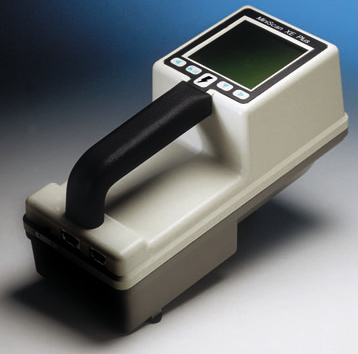
\includegraphics[scale=0.9]{img/MiniScanXEPlus}
			\caption{FIGURA 1. MiniScan XE Plus}
		\end{figure}
\vfill

\section{Resultados y Conclusiones}
	
	\subsection{Resultados}
	
	Para establecer la comunicaci\'{o}n entre el MiniScan XE Plus y el nuevo software, se recurri\'{o} a la documentaci\'{o}n del instrumento, en la cual se describe el MSXE.ocx \cite{MiniScanXEPlus-manual}, un archivo que implementa las funciones comunmente utilizadas por dicho instrumento. Se contact\'{o} al personal de soporte t\'{e}cnico de HunterLab por correo electr\'{o}nico, para solicitarle el c\'{o}digo fuente de dicho archivo y la documentaci\'{o}n relativa a su utilizaci\'{o}n que se pudiera proporcionar para la investigaci\'{o}n.
	
	Si bien el personal no comparti\'{o} el c\'{o}digo fuente del archivo, s\'{i} envi\'{o} la documentaci\'{o}n solicitada y un ejemplo de su uso escrito en Visual Basic for Applications (VBA). Primero se intent\'{o} cargar el archivo y utilizarlo directamente en Qt; sin embargo, ocurr\'{i}a un error de compatibilidad de datos al invocar algunas de sus funciones. La soluci\'{o}n a este problema fue desarrollar una librer\'{i}a escrita en Visual Basic .NET, con la cual se pueden invocar todas las funciones de este archivo sin problema alguno.

	As\'{i} pues, por medio del cable adaptador RS232-USB, y empleando la librer\'{i}a escrita en Visual Basic .NET, se logr\'{o} establecer la comunicaci\'{o}n entre el nuevo software y el MiniScan XE Plus.
	
	El software resultante, denominado Spectrasoft, se puede apreciar en la figura 2 con datos de ejemplo, as\'{i} como la gr\'{a}fica de la curva de reflectancia difusa de dichos datos en la figura 3. Este software resultante dispone de las funcionalidades listadas en la tabla 3.

\FloatBarrier

\begin{figure*}[h]
  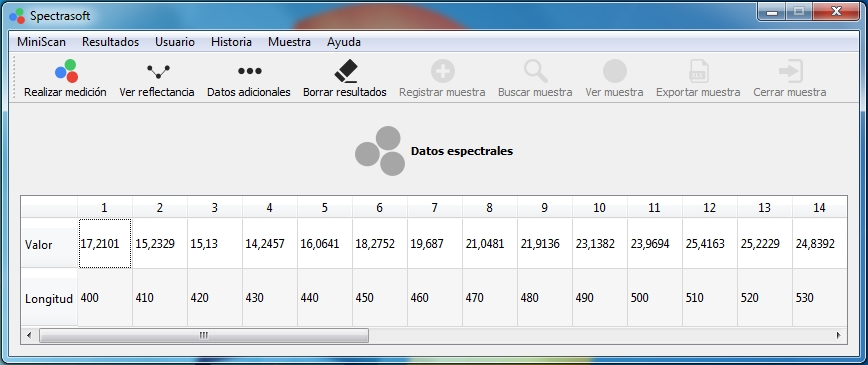
\includegraphics[scale=.8]{./img/spectrasoft.jpg}
  \caption{FIGURA 2. Vista principal del Spectrasoft}
\end{figure*}

\FloatBarrier

\begin{figure}[h]
  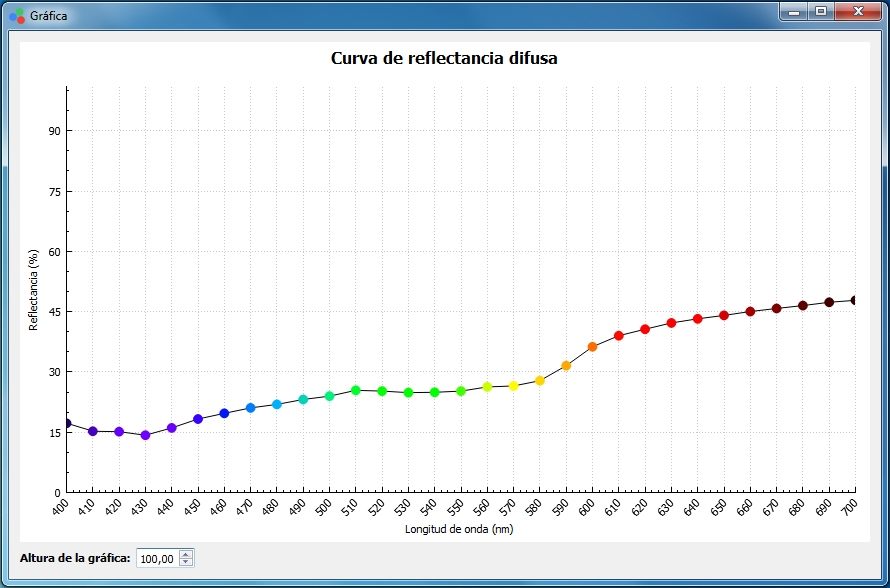
\includegraphics[scale=.375]{./img/curva-reflectancia.jpg}
  \caption{FIGURA 3. Curva de reflectancia difusa del Spectrasoft}
\end{figure}
	
\FloatBarrier
		\begin{table}[H]
			\caption{TABLA 3. Funcionalidades del Spectrasoft}
			\label{tabla_3}
			\centering
			\setlength{\extrarowheight}{2.5pt}
			\begin{tabulary}{8.8cm}{|c|J|}
				\hline
				\thead{\textbf{\#}} & \thead{\textbf{Funcionalidades}}\\ \hline
				1 & Conectar, desconectar y calibrar el MiniScan XE Plus.\\ \hline		
				2 & Realizar medici\'{o}n con el MiniScan XE Plus.\\ \hline
				
				3 & Mostrar los datos obtenidos de la medici\'{o}n con el MiniScan XE Plus.\\ \hline
				
				4 & Graficar las curvas de reflectancia difusa y de absorbancia aparente.\\ \hline
				
				5 & Calcular y graficar el coeficiente de absorci\'{o}n.\\
\hline
				6 & Calcular y mostrar las coordenadas de cromaticidad CIE xyz.\\ \hline
				
				7 & Calcular y mostrar las coordenadas del espacio CIELAB.\\ \hline
				
				8 & Calcular y mostrar el \'{i}ndice de eritema.\\ \hline

				9 & Gestionar la creaci\'{o}n, consulta, modificaci\'{o}n y eliminaci\'{o}n de los usuarios.\\ \hline
				
				10 & Gestionar la creaci\'{o}n, consulta, modificaci\'{o}n y eliminaci\'{o}n de las historias.\\ \hline

				11 & Gestionar la creaci\'{o}n, consulta, modificaci\'{o}n y eliminaci\'{o}n de las muestras.\\ \hline
				
				12 & Exportar los datos de una muestra a un archivo port\'{a}til.\\ \hline
			\end{tabulary}
		\end{table}
\FloatBarrier

	\subsection{Conclusiones}
	
	La interfaz gr\'{a}fica de usuario del Spectrasoft es sencilla y est\'{a} en espa\~{n}ol, por lo tanto es amigable. Se realiz\'{o} un manual de usuario para su utilizaci\'{o}n, que explica detalladamente y con im\'{a}genes la permisolog\'{i}a de sus usuarios y las funciones que ofrece, por lo que su curva de aprendizaje es baja. Fue desarrollado con herramientas y tecnolog\'{i}as actuales, por lo que puede ejecutarse en sistemas operativos Windows actuales, garantizando su utilizaci\'{o}n en los equipos disponibles en el CIMBUC. Por \'{u}ltimo, las funcionalidades que ofrece el Spectrasoft se adaptan a las necesidades de los dermat\'{o}logos.	

	En definitiva, se concluye que el Spectrasoft cumple con el objetivo de ajustarse a las necesidades de los dermat\'{o}logos, y garantizar\'{a} un mejor aprovechamiento del MiniScan XE Plus.
% conference papers do not normally have an appendix

% use section* for acknowledgement
\section*{Agradecimientos}
	Este trabajo de investigaci\'{o}n se llev\'{o} a cabo gracias a la tutor\'{i}a de los profesores Harold Vasquez y Patricia \mbox{Guerrero}, la orientaci\'{o}n del profesor Freddy Narea, la colaboraci\'{o}n del profesor Aar\'{o}n Mu\~{n}oz y de la doctora Sandra Vivas, al apoyo de todo el equipo de investigadores que hace vida en el CIMBUC, y finalmente a la ayuda proporcionada por el personal de soporte t\'{e}cnico de HunterLab.
	
	\textit{<<El hombre encuentra a Dios detr\'{a}s de cada puerta que la ciencia logra abrir>>} - Albert Einstein.

% trigger a \newpage just before the given reference
% number - used to balance the columns on the last page
% adjust value as needed - may need to be readjusted if
% the document is modified later
\IEEEtriggeratref{14}
% The "triggered" command can be changed if desired:
%\IEEEtriggercmd{\enlargethispage{-5in}}

% references section

% can use a bibliography generated by BibTeX as a .bbl file
% BibTeX documentation can be easily obtained at:
% http://www.ctan.org/tex-archive/biblio/bibtex/contrib/doc/
% The IEEEtran BibTeX style support page is at:
% http://www.michaelshell.org/tex/ieeetran/bibtex/
%\bibliographystyle{IEEEtran}
% argument is your BibTeX string definitions and bibliography database(s)
%\bibliography{IEEEabrv,../bib/paper}
%
% <OR> manually copy in the resultant .bbl file
% set second argument of \begin to the number of references
% (used to reserve space for the reference number labels box)
\begin{thebibliography}{1}

\bibitem{Bersha}
K.~S. Bersha, \emph{Spectral Imaging And Analysis Of Human Skin}.\hskip 1em plus
  0.5em minus 0.4em\relax Universidad del Este de Finlandia, 2010.

\bibitem{Perez}
A.~D. P\'{e}rez, \emph{Estudio de la Reflexi\'{o}n \'{O}ptica Difusa en Tejido Biol\'{o}gico}.\hskip 1em plus
  0.5em minus 0.4em\relax Escuela Superior de Ingenier\'{i}a Mec\'{a}nica y El\'{e}ctrica Unidad Zacatenco, 2012.

\bibitem{HunterLab}
Hunter Associates Laboratory, \emph{HunterLab, The World's true measure of color}.\hskip 1em plus
0.5em minus 0.4em\relax http://www.hunterlab.com/about-us.html.

\bibitem{HunterLab-manual}
\emph{Universal Software Versions 4.10 and Above User's Manual}.\hskip 1em plus
  0.5em minus 0.4em\relax Reston, Virginia: Hunter Associates Laboratory, 2001.

\bibitem{Sommerville}
I. Sommerville, \emph{Ingenier\'{i}a del Software}, 7ma~ed.\hskip 1em plus
  0.5em minus 0.4em\relax Madrid, Espa\~{n}a: Pearson Education, 2005.

\bibitem{Wagner}
J. Wagner et al., \emph{Comparing Quantitative Measures of Erythema, Pigmentation and Skin Response using Reflectometry}.\hskip 1em plus
  0.5em minus 0.4em\relax Pigment Cell Res, 2002.

\bibitem{Narea}
F. Narea et al., \emph{Recuperaci\'{o}n del coeficiente de absorci\'{o}n de la epidermis en la piel humana}.\hskip 1em plus
  0.5em minus 0.4em\relax Sociedad Espa\~{n}ola de \'{O}ptica, 2015.

\bibitem{Random}
\emph{Absorption spectrum. (n.d.) Random House Kernerman Webster's College Dictionary}.\hskip 1em plus
  0.5em minus 0.4em\relax K Dictionaries LTD, 2010.

\bibitem{CIE-report}
CIE, \emph{CIE 15: Technical Report: Colorimetry, 3rd edition}.\hskip 1em plus
0.5em minus 0.4em\relax Viena, Austria, 2004.

\bibitem{CIE}
CIE, \emph{Commission Internationale de l'Eclairage, International Commission on Illumination}.\hskip 1em plus
0.5em minus 0.4em\relax http://www.cie.co.at/index.php.

\bibitem{Schanda}
J. Schanda, \emph{Colorimetry: Understanding the CIE system}.\hskip 1em plus
  0.5em minus 0.4em\relax Hoboken, Nueva Jersey: John Wiley \& Sons, 2007.

\bibitem{Baskerville}
R.~L. Baskerville, \emph{Investigating Information Systems with Action Research}, vol~2.\hskip 1em plus
  0.5em minus 0.4em\relax Atlanta, GA: Association for Information Systems, 1999.

\bibitem{Schwaber&Sutherland}
K. Schwaber y J. Sutherland, \emph{The Definitive Guide to Scrum: The Rules of the Game}.\hskip 1em plus
  0.5em minus 0.4em\relax http://www.scrumguides.org/.

\bibitem{Kroll&Kruchten}
P. Kroll y P. Kruchten, \emph{The Rational Unified Process Made Easy: A Practitioner's Guide to the RUP}.\hskip 1em plus
  0.5em minus 0.4em\relax Addison-Wesley, 2003.

\bibitem{MiniScanXEPlus-manual}
\emph{MiniScan XE Plus User's Guide Version 2.4}.\hskip 1em plus
  0.5em minus 0.4em\relax Reston, Virginia: Hunter Associates Laboratory, 2006.

\bibitem{RS232}
Magneto Tech Research, \emph{USB to Serial adapters Wiki}.\hskip 1em plus
0.5em minus 0.4em\relax http://www.usb-serial-adapter.org/.

\bibitem{Qt}
The Qt Company, \emph{Qt, a Cross-Platform Framework for Application Development}.\hskip 1em plus
0.5em minus 0.4em\relax https://wiki.qt.io/About\_Qt.

\bibitem{VS}
Microsoft, \emph{Visual Studio Community, a fully-featured, extensible IDE}.\hskip 1em plus
0.5em minus 0.4em\relax https://www.visualstudio.com/products/visual-studio-community-vs.

\bibitem{PostgreSQL}
PostgreSQL, \emph{PostgreSQL: The world's most advanced open source database}.\hskip 1em plus
0.5em minus 0.4em\relax http://www.postgresql.org/about.

\bibitem{Gitlab}
Gitlab, \emph{Gitlab: Create, review, and deploy code together}.\hskip 1em plus
0.5em minus 0.4em\relax https://about.gitlab.com.

\bibitem{QCustomPlot}
QCustomPlot, \emph{A Qt C++ widget for plotting and data visualization}.\hskip 1em plus
0.5em minus 0.4em\relax http://www.qcustomplot.com/index.php/introduction.

\bibitem{Qtxlsx}
QtXlsx, \emph{A Qt library to read and write excel files that can be used in any platform that Qt5 supported}.\hskip 1em plus
0.5em minus 0.4em\relax http://www.qtxlsx.debao.me.

\end{thebibliography}

% that's all folks
\end{document}


